\documentclass{standalone}
\usepackage{tikz}
\usetikzlibrary{patterns, positioning}


\begin{document}
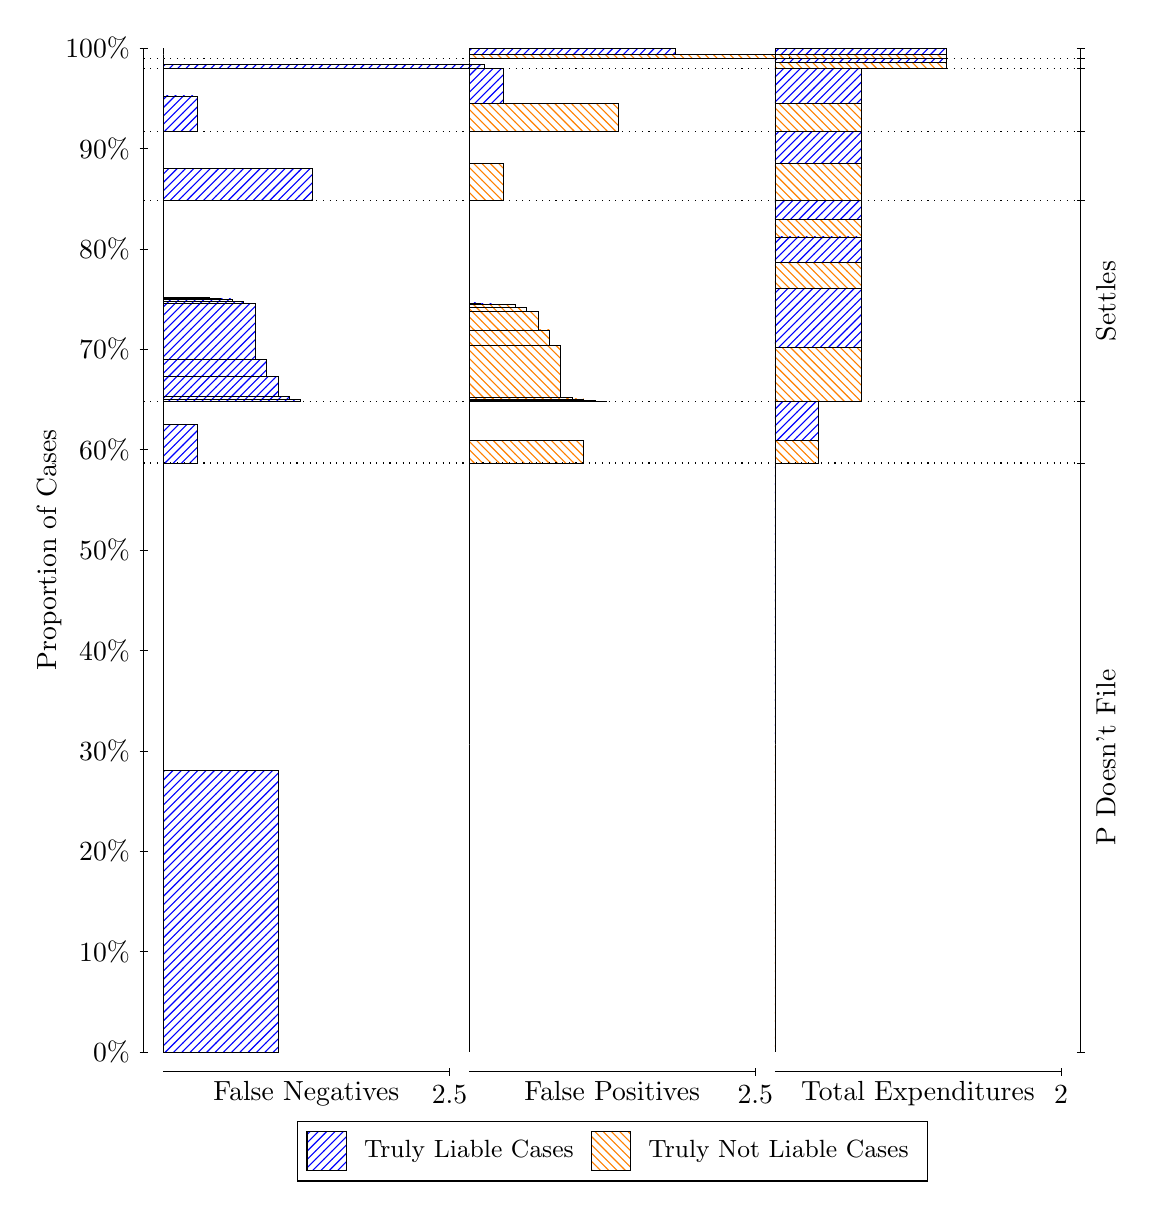
\begin{tikzpicture}
\draw[black, very thin] (1.5,1.75) -- (1.5,14.5);
\node[rotate=90, text=black, anchor=center] at (0.3, 8.125) {Proportion of Cases};
\draw[black, very thin] (1.45,1.75) -- (1.55,1.75);
\node[text=black, anchor=east] at (1.45, 1.75) {0\%};
\draw[black, very thin] (1.45,3.025) -- (1.55,3.025);
\node[text=black, anchor=east] at (1.45, 3.025) {10\%};
\draw[black, very thin] (1.45,4.3) -- (1.55,4.3);
\node[text=black, anchor=east] at (1.45, 4.3) {20\%};
\draw[black, very thin] (1.45,5.575) -- (1.55,5.575);
\node[text=black, anchor=east] at (1.45, 5.575) {30\%};
\draw[black, very thin] (1.45,6.85) -- (1.55,6.85);
\node[text=black, anchor=east] at (1.45, 6.85) {40\%};
\draw[black, very thin] (1.45,8.125) -- (1.55,8.125);
\node[text=black, anchor=east] at (1.45, 8.125) {50\%};
\draw[black, very thin] (1.45,9.4) -- (1.55,9.4);
\node[text=black, anchor=east] at (1.45, 9.4) {60\%};
\draw[black, very thin] (1.45,10.675) -- (1.55,10.675);
\node[text=black, anchor=east] at (1.45, 10.675) {70\%};
\draw[black, very thin] (1.45,11.95) -- (1.55,11.95);
\node[text=black, anchor=east] at (1.45, 11.95) {80\%};
\draw[black, very thin] (1.45,13.225) -- (1.55,13.225);
\node[text=black, anchor=east] at (1.45, 13.225) {90\%};
\draw[black, very thin] (1.45,14.5) -- (1.55,14.5);
\node[text=black, anchor=east] at (1.45, 14.5) {100\%};

\draw[black, very thin] (13.4,1.75) -- (13.4,14.5);
\draw[black, very thin] (13.35,1.75) -- (13.45,1.75);
\node[anchor=west] at (13.35, 1.75) {};
\draw[black, very thin] (13.35,9.2295) -- (13.45,9.2295);
\node[anchor=west] at (13.35, 9.2295) {};
\draw[black, very thin] (13.35,10.009) -- (13.45,10.009);
\node[anchor=west] at (13.35, 10.009) {};
\draw[black, very thin] (13.35,12.567) -- (13.45,12.567);
\node[anchor=west] at (13.35, 12.567) {};
\draw[black, very thin] (13.35,13.444) -- (13.45,13.444);
\node[anchor=west] at (13.35, 13.444) {};
\draw[black, very thin] (13.35,14.243) -- (13.45,14.243);
\node[anchor=west] at (13.35, 14.243) {};
\draw[black, very thin] (13.35,14.368) -- (13.45,14.368);
\node[anchor=west] at (13.35, 14.368) {};
\draw[black, very thin] (13.35,14.5) -- (13.45,14.5);
\node[anchor=west] at (13.35, 14.5) {};

\draw[black, very thin, pattern color=blue, pattern=north east lines] (1.75,1.75) rectangle (3.2033,5.3267);
\draw[black, very thin, pattern color=orange, pattern=north west lines] (1.75,5.3267) rectangle (1.75,9.2295);
\draw[black, very thin, pattern color=blue, pattern=north east lines] (1.75,9.2295) rectangle (2.186,9.7175);
\draw[black, very thin, pattern color=orange, pattern=north west lines] (1.75,9.7175) rectangle (1.75,10.009);
\draw[black, very thin, pattern color=blue, pattern=north east lines] (1.75,10.009) rectangle (3.494,10.038);
\draw[black, very thin, pattern color=blue, pattern=north east lines] (1.75,10.038) rectangle (3.3487,10.079);
\draw[black, very thin, pattern color=blue, pattern=north east lines] (1.75,10.079) rectangle (3.2033,10.329);
\draw[black, very thin, pattern color=blue, pattern=north east lines] (1.75,10.329) rectangle (3.058,10.335);
\draw[black, very thin, pattern color=blue, pattern=north east lines] (1.75,10.335) rectangle (3.058,10.545);
\draw[black, very thin, pattern color=blue, pattern=north east lines] (1.75,10.545) rectangle (2.9127,11.254);
\draw[black, very thin, pattern color=blue, pattern=north east lines] (1.75,11.254) rectangle (2.7673,11.282);
\draw[black, very thin, pattern color=blue, pattern=north east lines] (1.75,11.282) rectangle (2.622,11.314);
\draw[black, very thin, pattern color=blue, pattern=north east lines] (1.75,11.314) rectangle (2.4767,11.324);
\draw[black, very thin, pattern color=blue, pattern=north east lines] (1.75,11.324) rectangle (2.3313,11.335);
\draw[black, very thin, pattern color=orange, pattern=north west lines] (1.75,11.335) rectangle (1.75,12.567);
\draw[black, very thin, pattern color=blue, pattern=north east lines] (1.75,12.567) rectangle (3.6393,12.973);
\draw[black, very thin, pattern color=orange, pattern=north west lines] (1.75,12.973) rectangle (1.75,13.444);
\draw[black, very thin, pattern color=blue, pattern=north east lines] (1.75,13.444) rectangle (2.186,13.891);
\draw[black, very thin, pattern color=orange, pattern=north west lines] (1.75,13.891) rectangle (1.75,14.243);
\draw[black, very thin, pattern color=blue, pattern=north east lines] (1.75,14.243) rectangle (5.8193,14.292);
\draw[black, very thin, pattern color=orange, pattern=north west lines] (1.75,14.292) rectangle (1.75,14.368);
\draw[black, very thin, pattern color=orange, pattern=north west lines] (1.75,14.368) rectangle (1.75,14.418);
\draw[black, very thin, pattern color=blue, pattern=north east lines] (1.75,14.418) rectangle (1.75,14.5);
\draw[black, very thin, pattern color=orange, pattern=north west lines] (5.6333,1.75) rectangle (5.6333,5.6527);
\draw[black, very thin, pattern color=blue, pattern=north east lines] (5.6333,5.6527) rectangle (5.6333,9.2295);
\draw[black, very thin, pattern color=orange, pattern=north west lines] (5.6333,9.2295) rectangle (7.0867,9.5213);
\draw[black, very thin, pattern color=blue, pattern=north east lines] (5.6333,9.5213) rectangle (5.6333,10.009);
\draw[black, very thin, pattern color=orange, pattern=north west lines] (5.6333,10.009) rectangle (7.3773,10.016);
\draw[black, very thin, pattern color=orange, pattern=north west lines] (5.6333,10.016) rectangle (7.232,10.023);
\draw[black, very thin, pattern color=orange, pattern=north west lines] (5.6333,10.023) rectangle (7.0867,10.045);
\draw[black, very thin, pattern color=orange, pattern=north west lines] (5.6333,10.045) rectangle (6.9413,10.064);
\draw[black, very thin, pattern color=orange, pattern=north west lines] (5.6333,10.064) rectangle (6.796,10.725);
\draw[black, very thin, pattern color=orange, pattern=north west lines] (5.6333,10.725) rectangle (6.6507,10.92);
\draw[black, very thin, pattern color=orange, pattern=north west lines] (5.6333,10.92) rectangle (6.5053,11.16);
\draw[black, very thin, pattern color=orange, pattern=north west lines] (5.6333,11.16) rectangle (6.36,11.21);
\draw[black, very thin, pattern color=orange, pattern=north west lines] (5.6333,11.21) rectangle (6.2147,11.241);
\draw[black, very thin, pattern color=blue, pattern=north east lines] (5.6333,11.241) rectangle (5.924,11.252);
\draw[black, very thin, pattern color=blue, pattern=north east lines] (5.6333,11.252) rectangle (5.7787,11.263);
\draw[black, very thin, pattern color=blue, pattern=north east lines] (5.6333,11.263) rectangle (5.6333,12.567);
\draw[black, very thin, pattern color=orange, pattern=north west lines] (5.6333,12.567) rectangle (6.0693,13.037);
\draw[black, very thin, pattern color=blue, pattern=north east lines] (5.6333,13.037) rectangle (5.6333,13.444);
\draw[black, very thin, pattern color=orange, pattern=north west lines] (5.6333,13.444) rectangle (7.5227,13.795);
\draw[black, very thin, pattern color=blue, pattern=north east lines] (5.6333,13.795) rectangle (6.0693,14.243);
\draw[black, very thin, pattern color=orange, pattern=north west lines] (5.6333,14.243) rectangle (5.6333,14.319);
\draw[black, very thin, pattern color=blue, pattern=north east lines] (5.6333,14.319) rectangle (5.6333,14.368);
\draw[black, very thin, pattern color=orange, pattern=north west lines] (5.6333,14.368) rectangle (9.7027,14.418);
\draw[black, very thin, pattern color=blue, pattern=north east lines] (5.6333,14.418) rectangle (8.2493,14.5);
\draw[black, very thin, pattern color=orange, pattern=north west lines] (9.5167,1.75) rectangle (9.5167,5.6527);
\draw[black, very thin, pattern color=blue, pattern=north east lines] (9.5167,5.6527) rectangle (9.5167,9.2295);
\draw[black, very thin, pattern color=orange, pattern=north west lines] (9.5167,9.2295) rectangle (10.062,9.5213);
\draw[black, very thin, pattern color=blue, pattern=north east lines] (9.5167,9.5213) rectangle (10.062,10.009);
\draw[black, very thin, pattern color=orange, pattern=north west lines] (9.5167,10.009) rectangle (10.607,10.698);
\draw[black, very thin, pattern color=blue, pattern=north east lines] (9.5167,10.698) rectangle (10.607,11.45);
\draw[black, very thin, pattern color=orange, pattern=north west lines] (9.5167,11.45) rectangle (10.607,11.775);
\draw[black, very thin, pattern color=blue, pattern=north east lines] (9.5167,11.775) rectangle (10.607,12.102);
\draw[black, very thin, pattern color=orange, pattern=north west lines] (9.5167,12.102) rectangle (10.607,12.319);
\draw[black, very thin, pattern color=blue, pattern=north east lines] (9.5167,12.319) rectangle (10.607,12.567);
\draw[black, very thin, pattern color=orange, pattern=north west lines] (9.5167,12.567) rectangle (10.607,13.037);
\draw[black, very thin, pattern color=blue, pattern=north east lines] (9.5167,13.037) rectangle (10.607,13.444);
\draw[black, very thin, pattern color=orange, pattern=north west lines] (9.5167,13.444) rectangle (10.607,13.795);
\draw[black, very thin, pattern color=blue, pattern=north east lines] (9.5167,13.795) rectangle (10.607,14.243);
\draw[black, very thin, pattern color=orange, pattern=north west lines] (9.5167,14.243) rectangle (11.697,14.319);
\draw[black, very thin, pattern color=blue, pattern=north east lines] (9.5167,14.319) rectangle (11.697,14.368);
\draw[black, very thin, pattern color=orange, pattern=north west lines] (9.5167,14.368) rectangle (11.697,14.418);
\draw[black, very thin, pattern color=blue, pattern=north east lines] (9.5167,14.418) rectangle (11.697,14.5);
\draw[black, dotted] (1.5,9.2295) -- (13.4,9.2295);
\draw[black, dotted] (1.5,10.009) -- (13.4,10.009);
\draw[black, dotted] (1.5,12.567) -- (13.4,12.567);
\draw[black, dotted] (1.5,13.444) -- (13.4,13.444);
\draw[black, dotted] (1.5,14.243) -- (13.4,14.243);
\draw[black, dotted] (1.5,14.368) -- (13.4,14.368);
\draw[black, very thin] (1.75,1.5) -- (5.3833,1.5);
\node[text=black, anchor=north] at (3.5667, 1.5) {False Negatives};
\draw[black, very thin] (5.3833,1.45) -- (5.3833,1.55);
\node[text=black, anchor=north] at (5.3833, 1.45) {2.5};

\draw[black, very thin] (5.6333,1.5) -- (9.2667,1.5);
\node[text=black, anchor=north] at (7.45, 1.5) {False Positives};
\draw[black, very thin] (9.2667,1.45) -- (9.2667,1.55);
\node[text=black, anchor=north] at (9.2667, 1.45) {2.5};

\draw[black, very thin] (9.5167,1.5) -- (13.15,1.5);
\node[text=black, anchor=north] at (11.333, 1.5) {Total Expenditures};
\draw[black, very thin] (13.15,1.45) -- (13.15,1.55);
\node[text=black, anchor=north] at (13.15, 1.45) {2};

\node[text=black, centered, rotate=90] at (13.72, 5.4897) {P Doesn't File};

\node[text=black, centered, rotate=90] at (13.72, 11.288) {Settles};





\draw (7.449999999999999,1.5) node[draw=none] (baseCoordinate) {};
\begin{scope}[align=center]
        \matrix[scale=0.5, draw=black, below=0.5cm of baseCoordinate, nodes={draw}, column sep=0.1cm]{
            \node[rectangle, draw, minimum width=0.5cm, minimum height=0.5cm, pattern color=blue, pattern=north east lines] {}; &
            \node[draw=none, font=\small, text=black] (B) {Truly Liable Cases}; &
            \node[rectangle, draw, minimum width=0.5cm, minimum height=0.5cm, pattern color=orange, pattern=north west lines] {}; &
            \node[draw=none, font=\small, text=black] (B) {Truly Not Liable Cases}; \\
            };
\end{scope}

\end{tikzpicture}
\end{document}